\documentclass[12pt]{article}
\usepackage{./common/karnaugh-map}
\usepackage{scrextend}
\usepackage[utf8]{inputenc}
\usepackage[polish]{babel}
\usepackage[T1]{fontenc}%polskie znaki
\usepackage[utf8]{inputenc}%polskie znaki
\usepackage{geometry}
\usepackage{float}
\usepackage{enumitem}
\usepackage{hyperref}
\usepackage{graphicx}
\usepackage{tabulary}
\usepackage{etoc}
\usepackage[normalem]{ulem} 
\renewcommand{\baselinestretch}{1.5}
\graphicspath{ {img/} }
\newgeometry{lmargin=2.5cm, rmargin=2.5cm, tmargin=2.5cm, bmargin=2.5cm}
\usepackage{tikz}
\usepackage[bf]{caption}
\usepackage{subcaption}
\usepackage{amsmath}
\usepackage{listings}
\usepackage{tikz}

\usepackage{tikz-timing}
\definecolor{codegreen}{rgb}{0,0.6,0}
\definecolor{codegray}{rgb}{0.5,0.5,0.5}
\definecolor{codepurple}{rgb}{0.58,0,0.82}
\definecolor{backcolour}{rgb}{0.95,0.95,0.93}
 
\lstdefinestyle{mystyle}{
    backgroundcolor=\color{backcolour},   
    commentstyle=\color{codegreen},
    keywordstyle=\color{magenta},
    numberstyle=\tiny\color{codegray},
    stringstyle=\color{codepurple},
    basicstyle=\ttfamily\footnotesize,
    breakatwhitespace=false,         
    captionpos=b,                    
    keepspaces=true,                 
    numbers=left,                    
    numbersep=5pt,                  
    showspaces=false,                
    showstringspaces=false,
    showtabs=false,                  
    tabsize=2,
    breaklines=true,
    postbreak=\mbox{\textcolor{red}{$\hookrightarrow$}\space},
}
\lstset{style=mystyle}

\title{ 
    \vspace*{50mm}
    \textsc{
        \textbf{Układy Cyfrowe i Systemy Wbudowane 2}\\
        \large Projekt \\
         Organy z pozytywką
    }
} 
\author{
Maja Bojarska, 241287\\
Damian Koper,  241292\\
}

\date{\today}

\begin{document}

\maketitle

\newpage

\section{Cel projektu}

Celem projektu było wykonanie układu realizujący działanie organów sterowanych za pomocą klawiszy klawiatury podłączonej z wykorzystaniem interfejsu PS2. Rozszerzeniem działania układu było odtwarzanie sekwencji dźwięków zapisanej w pliku tesktowym odczytanych z~karty pamięci SD.

\subsection{Założenia wstępne}

Początkowy projekt układu zakładał podział kolejnych funkcjonalności na możliwie małe moduły według zasady pojedynczej odpowiedzialności. Układ mapował klawisze klawiatury na właściwe tony. Klawisze były przypisane w przybliżeniu zgodnie z układem klawiszy pianina.  Klawisze A -- J odpowiadały tonom C -- H, a klawisze W -- E i T -- U półtonom kolejno C\# -- D\# i F\# -- A\#. Oktawa zmieniana była za pomocą klawiszy strzałek w zakresie od 0 do 8.

Pierwotny projekt zawierał również podziała na wiele typów fal, których zmiana dokonywana być miała pomocą sygnałów z enkodera. Diagram przepływu danych wstępnego projektu przedstawia rysunek \ref{base}.
% TODO: Może da się to ładniej napisać

\begin{figure}[H]
  \centering
  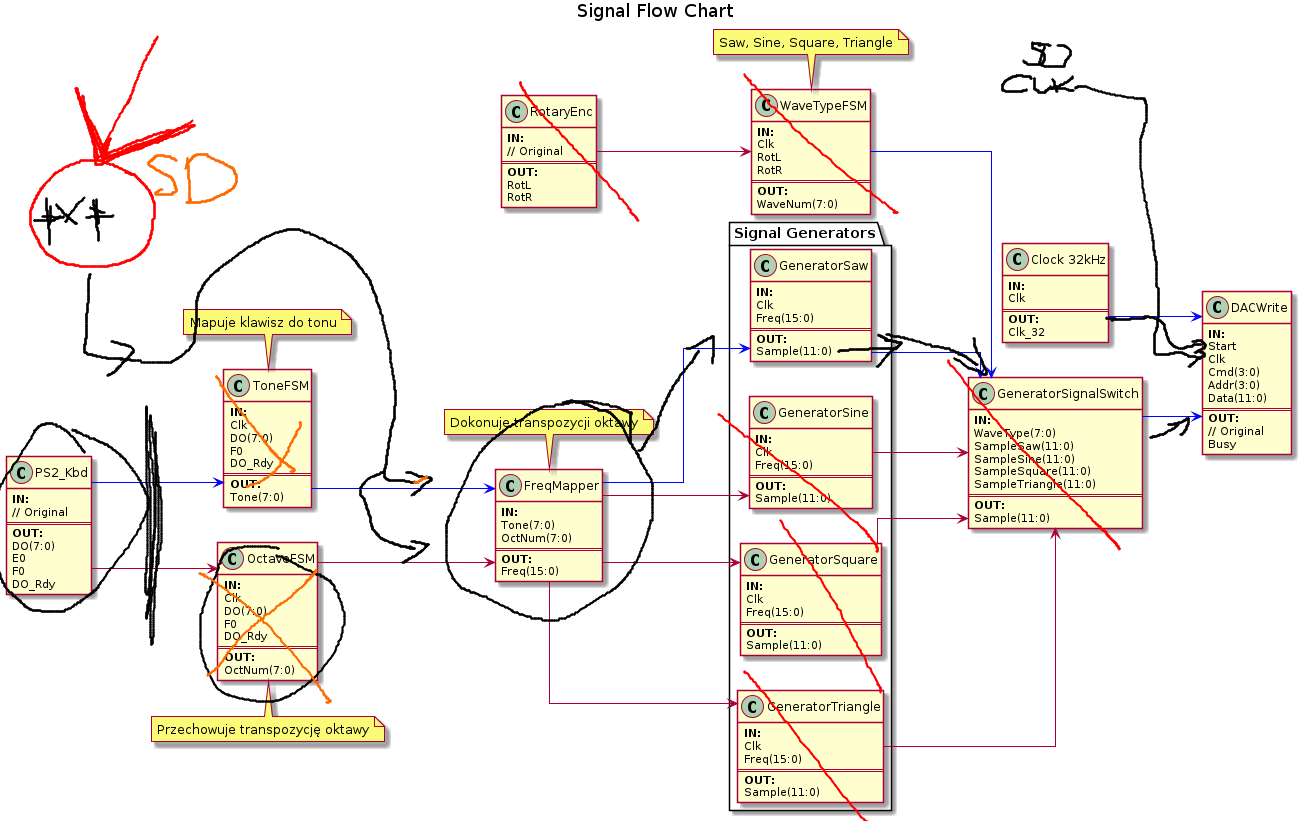
\includegraphics[width=\linewidth]{./diagram/out/flow_chart}
  \caption{Bazowy projekt organów. Niebieskimi strzałkami oznaczono podstawową i~wykonaną jako pierwszą funkcjonalność. }
  \label{base}
\end{figure}

\subsection{Założenia rozszerzone}

Rozszerzeniem funkcjonalności organów sterowanych za pomocą klawiatury było uzyskanie możliwości odtwarzania wcześniej zapisanej sekwencji dźwięków o~zmiennej długości. Wykorzystano do tego możliwość wczytania danych z karty pamięci i moduł \textit{SDC\_FileReader}.
Przykład zapisu dźwięku w pliku tekstowym:
\begin{align*}
  a40000000101001101
\end{align*}
gdzie:
\begin{align*}
  a                & - Ton                    \\
  4                & - Oktawa                 \\
  0000000101001101 & - Czas\;trwania\;[x*3ms] \\
\end{align*}
Jeden dźwięk jest definiowany zawsze z wykorzystaniem 18 znaków, więc zapis nie wymaga stosowania separatorów. Czas trwania dźwięku zapisany jest z wykorzystaniem liczby binarnej zapisanej tekstowo na 16 bitach i definiuje czas trwania jako wielokrotność $3ms$.

\section{Struktura układu}
\subsection{Schemat najwyższego poziomu}
Schemat najwyższego poziomu przedstawiony na rysunku \ref{sch:main} zawiera wszystkie zawnętrzne moduły odpowiedzialne za komunikację z urządzeniami peryferyjnymi. Są to:
\begin{itemize}[noitemsep]
  \item \textit{SDC\_FileReader}
  \item \textit{PS2\_Kbd}
  \item \textit{DACWrite}
\end{itemize}
Wszystkie moduły komunikują się z modułem \textit{InnerLogic}.


\begin{figure}[h]
  \centering
  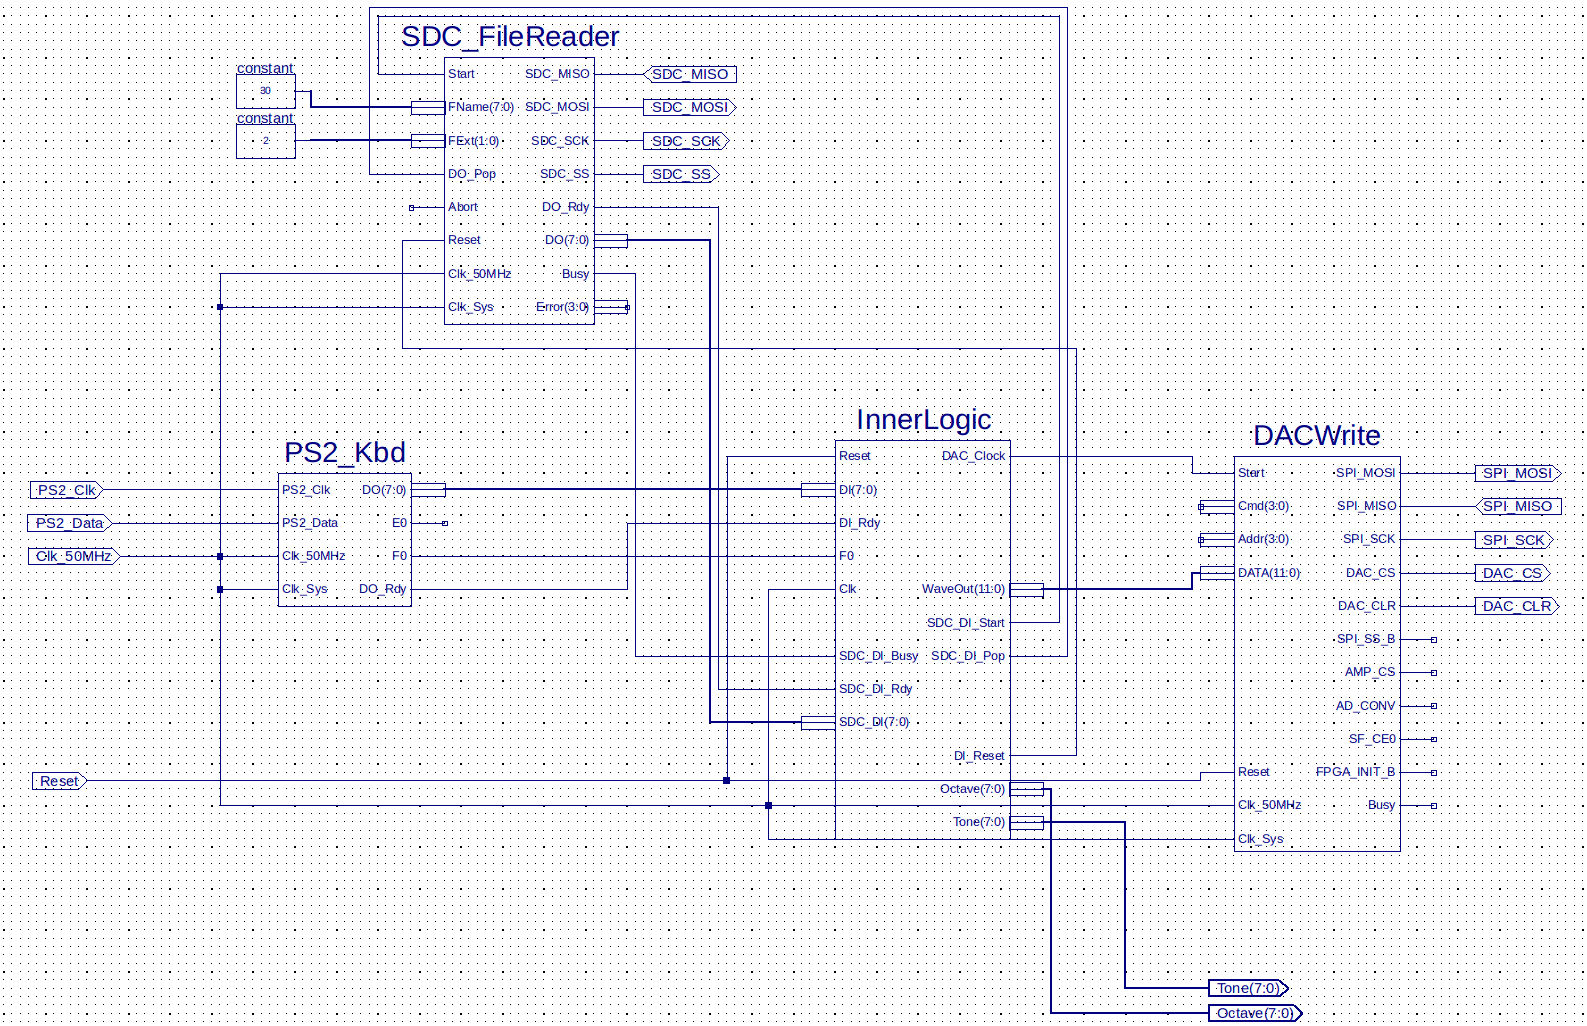
\includegraphics[width=\linewidth]{images/main}
  \caption{Schemat najwyższego poziomu.}
  \label{sch:main}
\end{figure}

\subsection{InnerLogic}

Schemat InnerLogic przedstawiony na rysunku \ref{sch:inner} zawiera wszystkie moduły odpowiedzialne za generowanie sygnału wyjściowego na podstawie danych wejściowych zebranych z klawiatury i karty SD. Przedstawione tutaj moduły mają swoje częściowe odwzorowanie we wstępnym projekcie przedstawionym na rysunku \ref{base}.

% TODO: Maja upodate zdemcie bo nie ma OctaveFSM
\begin{figure}[h]
  \centering
  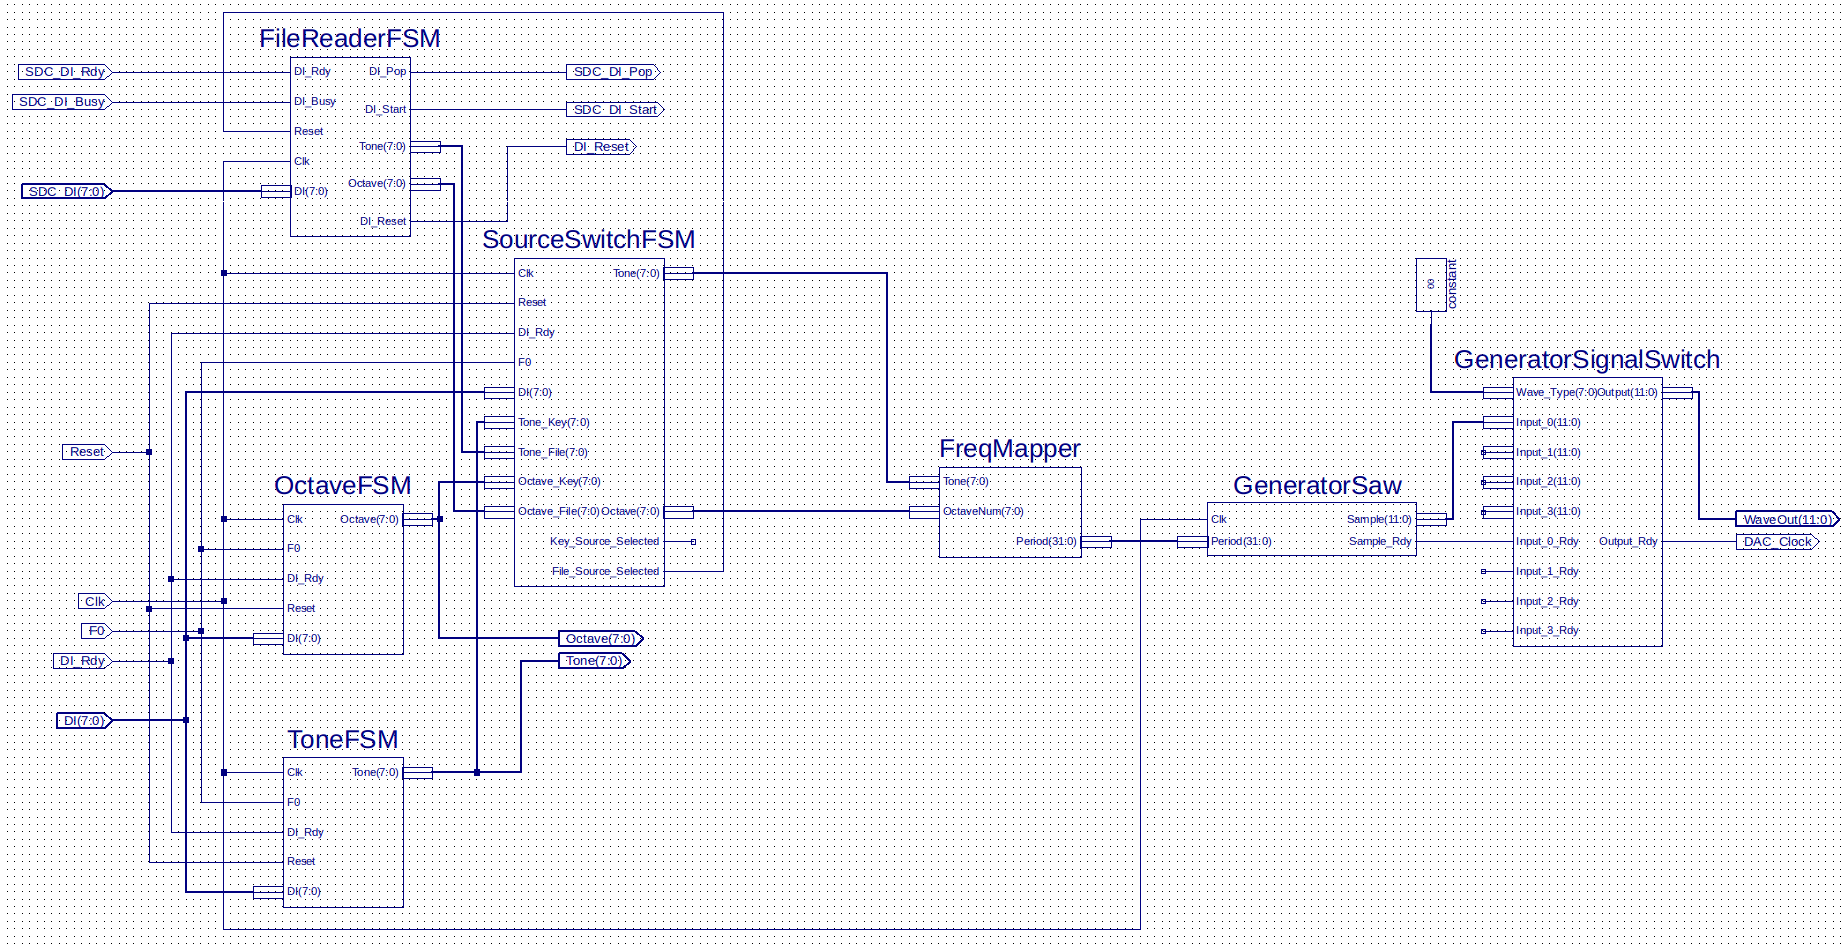
\includegraphics[width=\linewidth]{images/inner}
  \caption{Schemat InnerLogic.}
  \label{sch:inner}
\end{figure}

\subsection{FileReaderFSM}

Moduł FileReaderFSM realizuje maszynę stanów, która odpowiedzialna jest za interakcje z modułem \textit{SDC\_FileReader}. Odpowiada on za dostarczanie numeru tonu i oktawy przez określony czas, gdzie wszystkie te dane odczytywane są z karty SD.

Moduł \textit{SDC\_FileReader} umożliwia obsługę odczytu jako obsługę kolejki FIFO. Moduł \textit{FileReaderFSM} w procesie odczytu danych jednego dźwięku odczytuje najpierw znak tonu, potem oktawy, a następnie czas jego trwania wpisując tę wartość do licznika. Po zakończonym odczycie 18 znaków licznik jest uruchamiany, a zmapowane kody tonu i oktawy są widoczne na wyjściu dopóki licznik się nie wyzeruje. Wczytanie tonu $1$ i oktawy $4$ przedstawia symulacja na rysynku \ref{sim:fileReader}.

Ton i oktawa podawane są na wyjście zaraz po ich odczytaniu, a licznik uruchamiany jest po wczytaniu całego słowa określającego długość dźwięku. Skutkuje to pomijalnie małym wydłużeniem czasu trwania dźwięku.

\begin{figure}[h]
  \centering
  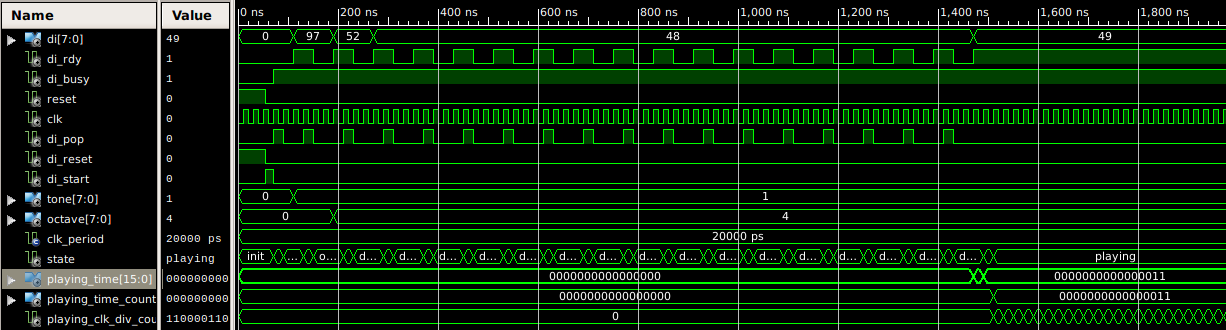
\includegraphics[decodearray={1 0 1 0 1 0}, width=\linewidth]{images/filereader}
  \caption{Symulacja modułu FileReaderFSM.}
  \label{sim:fileReader}
\end{figure}

\subsection{ToneFSM}
ToneFSM realizuje maszynę stanów, której stan określa aktualnie odtwarzany ton.
Kody od 1 do % TODO: ile xd
xd odpowiadają wszystkim tonom i półtonom jednej oktawy. Kod 0 odpowiada ciszy, czyli stanowi, kiedy żaden przycisk nie jest wciśnięty. Stan maszyny zmieniany jest w momencie naciśnięcia lub puszczenia przycisku na klawiaturze i stan ten następnie jest mapowany na odpowiedni kod tonu. Kolejne wciśnięcia przycisków (a, w, s, e, d, r, f) przedstawia symulacja na rysunku \ref{sim:tone}.

\begin{figure}[h]
  \centering
  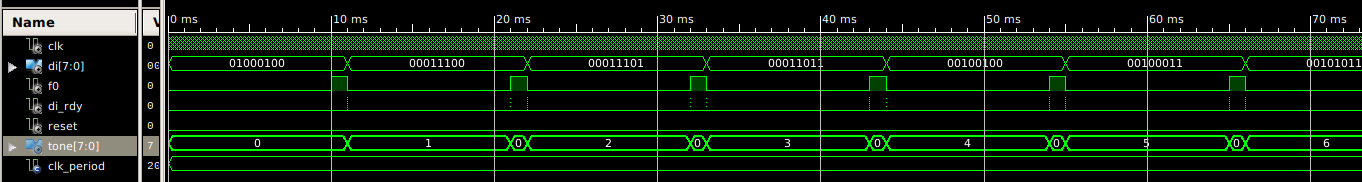
\includegraphics[decodearray={1 0 1 0 1 0}, width=\linewidth]{images/tone}
  \caption{Symulacja modułu ToneFSM.}
  \label{sim:tone}
\end{figure}
\subsection{OctaveFSM}
% Maja zrup
xd
\subsection{SourceSwitchFSM}
Moduł SourceSwitchFSM odpowiedzialny jest za wybór źródła dźwięku i za restartowanie odczytu dźwięków z karty pamięci w przypadku wyboru tego źródła. Klawisz M zmienia źródło na klawiaturę, a klawisz N na kartę pamięci. Na symulacji z rysunku \ref{sim:source} widać zmianę domyślnego źródła klawiatury na kartę pamięci i wysłanie impulsu wystąpienia zdarzenia zmiany źródła. Zdarzenie to obsługiwane jest przez moduł \textit{FileReaderFSM}, który restartuje proces odczytu.
\begin{figure}[h]
  \centering
  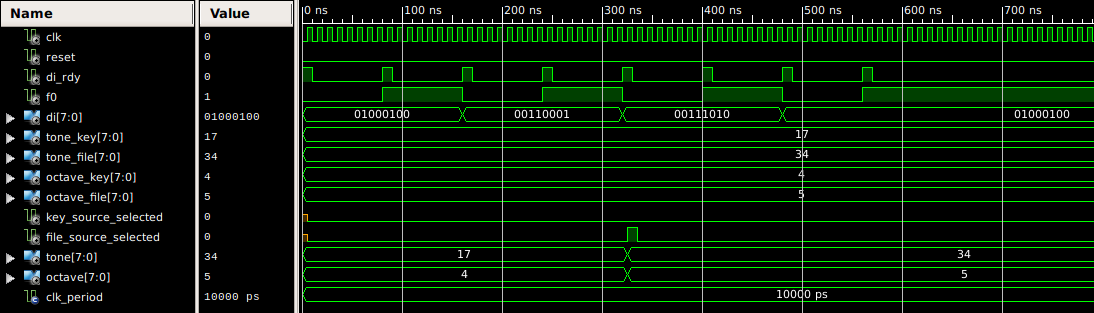
\includegraphics[decodearray={1 0 1 0 1 0}, width=\linewidth]{images/source}
  \caption{Symulacja modułu SourceSwitchFSM.}
  \label{sim:source}
\end{figure}
\subsection{FreqMapper}
FreqMapper obsługuje proces mapowania oktawy i tonu na liczbę cykli zegara o częstotliwości 50MHz, która odpowiada okresowi fali danego dźwięku. Ton 0 mapowany jest zawsze na wartość 0, co w dalszym procesie generowania sygnału oznacza ciszę. Symulację dla oktawy 0 i 3 przedstawia rysunek \ref{sim:mapper}.
\begin{figure}[h]
  \centering
  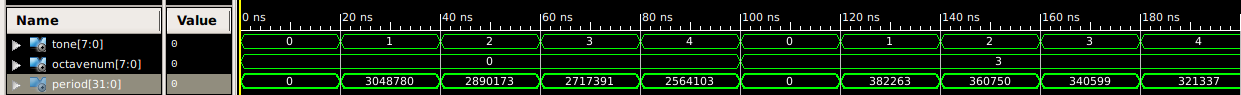
\includegraphics[decodearray={1 0 1 0 1 0}, width=\linewidth]{images/mapper}
  \caption{Symulacja modułu FreqMapper.}
  \label{sim:mapper}
\end{figure}
% TODO Maja weź tutaj jakieś przykłądowe przeliczenie z symulacji
% czyli np 382263 -matma x 50Mhz-> xyz Hz => dźwięk c4, qmasz nie?

\subsection{GeneratorSaw}
% MAja zrup
xd
\subsection{GeneratorSignalSwitch}
% MAja zrup
xd

\section{Symulacja InnerLogic}
Oba warianty wejść zostały odpowiednio przetestowane w symulacji. Rysuneki \ref{sim:kb} i \ref{sim:sd} przedstawiają symulacje działania modułu InnerLogic i falę generowaną przez ten moduł.
\subsection{Wejście z klawiatury}
Rysunek \ref{sim:kb} przedstawia symulację działania modułu InnerLogic i falę generowaną przez ten moduł. Symulacja obejmuje odtworzenie wszystkich tonów poprzez wciśnięcie odpowiadających im klawiszy. Przeplatane jest to chwilą ciszy, co widać na symulacji.
\begin{figure}[h]
  \centering
  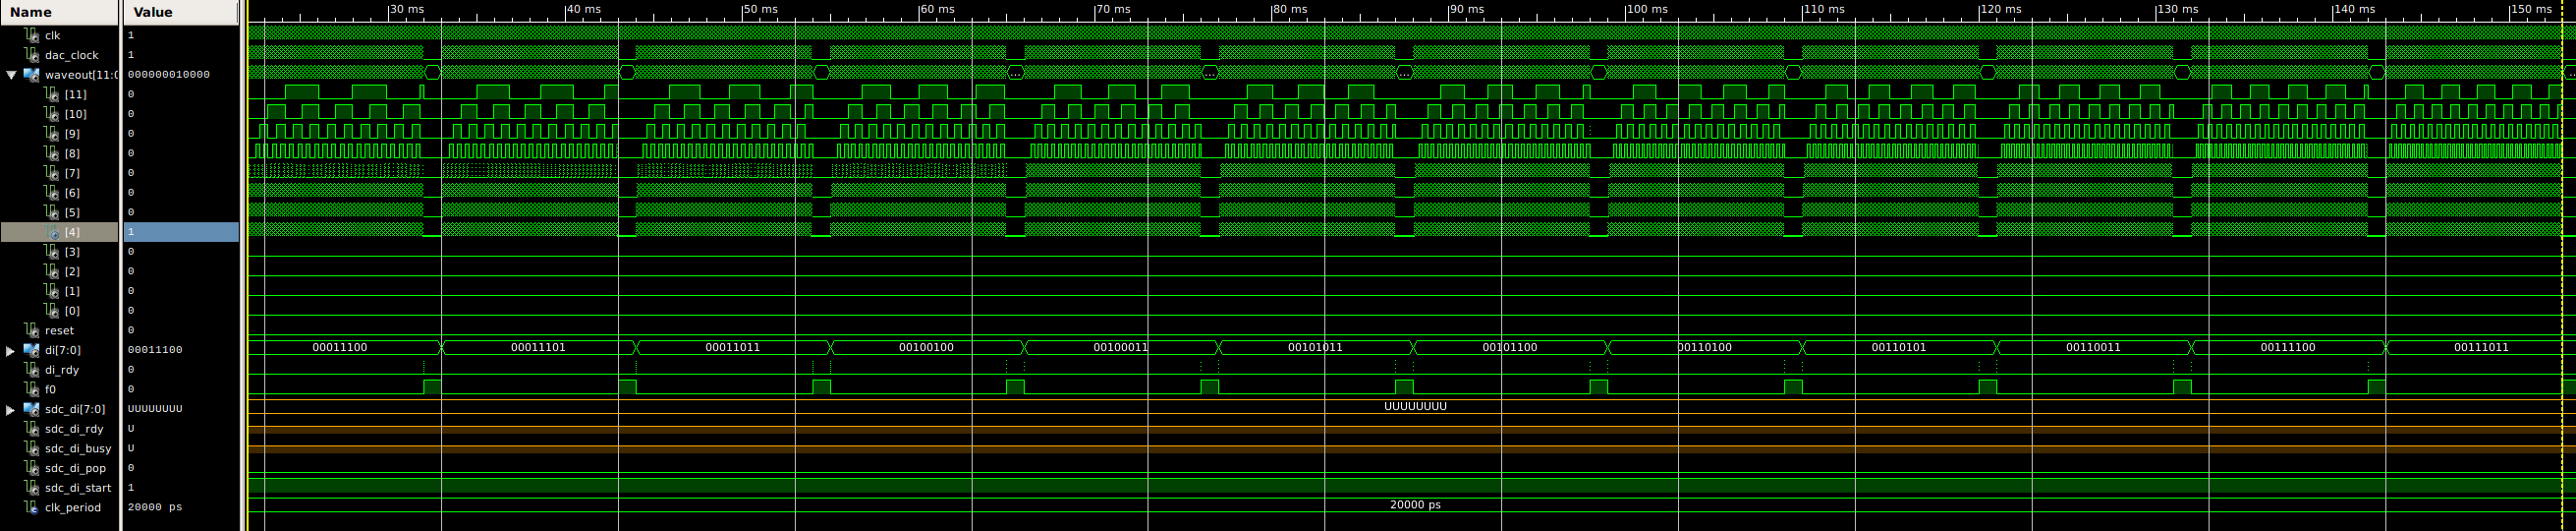
\includegraphics[decodearray={1 0 1 0 1 0}, width=\linewidth]{images/inner_sim_kb}
  \caption{Symulacja modułu InnerLogic. Wejście z klawiatury.}
  \label{sim:kb}
\end{figure}

\subsection{Wejście z karty pamięci}
 Symulacja obejmuje odtworzenie melodii zdefiniowanej w pliku na karcie pamięci. Dźwięki opisane są następującym ciągiem:
 \begin{lstlisting}
  a40000000000000001w40000000000000001s40000000000000001 e40000000000000001d40000000000000001f40000000000000001 t40000000000000001g40000000000000001y40000000000000001 h40000000000000001u40000000000000001j40000000000000001
 \end{lstlisting}
\begin{figure}[h]
  \centering
  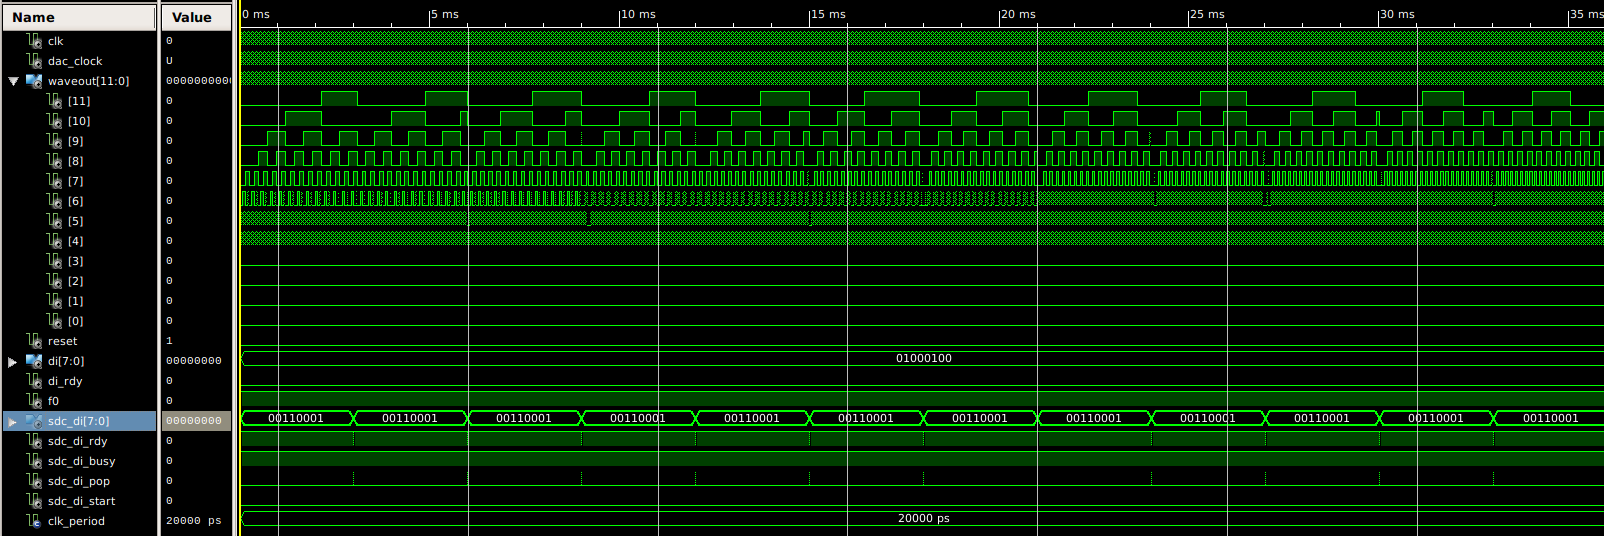
\includegraphics[decodearray={1 0 1 0 1 0}, width=\linewidth]{images/inner_sim_sd}
  \caption{Symulacja modułu InnerLogic. Wejście z karty pamięci.}
  \label{sim:sd}
\end{figure}

\section{Podsumowanie}
\subsection{Analiza czasów}
Narzędzie ISE w wygenerowanym raporcie z procesu implementacji zapewnił, że wymagania czasowe związane z częstotliwością taktowania zegara 50MHz zostaną spełnione.
\begin{lstlisting}
Timing summary: 
--------------- 
Timing errors: 0  Score: 0  (Setup/Max: 0, Hold: 0) 
Constraints cover 5434354 paths, 0 nets, and 7551 connections 
Design statistics: 
   Minimum period:  17.917ns{1}   (Maximum frequency:  55.813MHz) 
\end{lstlisting}

\subsection{Zrealizowane założenia}
Działanie poparte poprawnymi efektami symulacji pozwala sądzić, iż projekt został wykonany poprawnie zgodnie ze wstępnymi założeniami. Zrezygnowano jednak z pozostałych generatorów typów fal, pozostając tylko przy fali piłokształtnej, ponieważ proces generowania fali w pozostałych generatorach odbywałby się podobnie. Czy to poprzez użycie innego zachowania liczników, czy to poprzez podawanie na wyjście stablicowanych wartości.


\end{document}